% Functional specification for ProfiSnort
\documentclass[a4paper]{scrreprt}

\usepackage[german]{babel}
\usepackage[utf8]{inputenc}
\usepackage[T1]{fontenc}
\usepackage{ae}
\usepackage[bookmarks,bookmarksnumbered]{hyperref}
\usepackage{csquotes}
\usepackage{longtable}
\usepackage{enumitem, hyperref}
\usepackage{graphicx}

\usepackage{xcolor}
\hypersetup{
    colorlinks,
    linkcolor={red!50!black},
    citecolor={blue!50!black},
    urlcolor={blue!80!black}
}

\usepackage[ampersand]{easylist}

\makeatletter
\def\namedlabel#1#2{\begingroup
    #2%
    \def\@currentlabel{#2}%
    \phantomsection\label{#1}\endgroup
}
\makeatother

\newcommand{\sppname}{spp\_profinet }
\newcommand{\programname}{Netzwerk.IO }

\begin{document}

\title{\programname \& \sppname --- Pflichtenheft}
\author{
    Brendl, Julian
    \texttt{ubems@student.kit.edu}
    \and
    Diez, Maximilian
    \texttt{maximilian.diez@student.kit.edu}
    \and
    Giraud, Mark
    \texttt{mark.giraud@student.kit.edu}
    \and
    Hermes, Jan
    \texttt{jan.hermes@student.kit.edu}
    \and
    Höhler, Dimitri
    \texttt{mail@student.kit.edu}
    \and
    Kiechle, Valentin
    \texttt{mail@student.kit.edu}
}
\maketitle

\chapter{Einleitung} 
Dieses Dokument dient der genaueren Beschreibung und Dokumentation des Entwurfs zum Visualisierungstool Trufflehog, dessen Hauptaufgabe die Darstellung des Netzwerkverkehrs eines ProfiNet-Systems ist. Des Weiteren wird der im IDS Snort eingebaute Präprozessor \sppname und die genaue Funktionsweise der Inter-Prozess-Kommunikation (im Folgenden IPC) zu Trufflehog genau erläutert.

Das Design von Trufflehog baut auf dem klassischen Model-View-Controller (im Folgenden MVC) auf und erweitert diesen Entwurf zu einem Model-View-Presenter mit zusätzlicher Funktionalität.

//hier MVC von Präsentation und ähnliches Bild zum aktuellen Entwurf einfügen//


\newpage
\tableofcontents
\newpage

\chapter{Zielbestimmung}

Profisnort und PSAnalyzer sollen eine Möglichkeit schaffen, das Intrusion-Detection-System Snort auch mit ProfiNET verwenden zu können.
Hierbei soll PSAnalyzer eine übersichtliche Darstellung der Beziehungen und Datenflüsse in dem überwachten Netzwerk bieten.

\section{Musskriterien}

\subsection{spp\_profinet (Snort Präprozessor)}

\begin{itemize}
\item Der Präprozessor muss Ethernet-ProfiNet-Pakete erkennen und dekodieren können.

\item Der Präprozessor muss ein Ausgabeinterface bereitstellen damit Netzwerk.IO die dekodierten Paketdaten empfangen und weiterverarbeiten kann.

\item Der Präprozessor muss die PROFINET Header Daten zusammenfassen und an Netzwerk.IO weitergeben.
\end{itemize}

\subsection{Netzwerk.IO (Analyseprogramm)}

\begin{itemize}
\item Das Analyseprogramm muss eine grafische Oberfläche mit folgenden Funktionen bieten:

\item Übersichtliche, dynamische Graph-Darstellung der einzelnen Komponenten eines Netzwerks.

\item Möglichkeit zur zusätzlichen Darstellung von detaillierten Informationen.

\item Legale und illegale Kommunikation müssen unterschiedlich dargestellt werden.

\item Möglichkeit, den Graphen zu skalieren.

\item Über ein Einstellungsmenü sollen Darstellungsvarianten spezifiziert werden können.

\item Das Analyseprogramm muss die Möglichkeit zur Datenhaltung für möglich spätere Auswertung bieten.
\end{itemize}

\section{Kannkritierien}

\subsection{spp\_profinet}

\begin{itemize}

\item Der Präprozessor kann decodierte Pakete Snort zur Verfügung stellen, damit sie dort weiterverarbeitet werden können. 

\item Der Präprozessor kann ProfiNET TCP Pakete erkennen und dekodieren.

\item Der Präprozessor ist in der Lage andere Protokollarten zur Weiterverarbeitung an Netzwerk.IO weiterzugeben.
\end{itemize}

\subsection{Netzwerk.IO}

\begin{itemize}
\item Es gibt ein Einstellungsmenü welches dem Nutzer ermöglicht grundlegende Einstellungen vorzunehmen.

\item Das Analysetool kann dem Nutzer grafische Statistiken des bisher stattgefundenen Netzwerkverkehrs anzeigen.

\item Das Analysetool kann von Snort ausgelöste Alerts im Graph darstellen.

\item Die Kommunikationswege und -richtungen können im Graphen dargestellt werden.

\item Der Paketdurchsatz kann im Graph dargestellt werden (z. B. Farbe der Kante)

\item Der Übertragungstyp kann, soweit bekannt, im Graph dargestellt werden. 

\item Ausgabe eines Kommunikationslogs bei Klicken auf eine Kante zwischen zwei Netzkomponenten.

\item Dem Benutzer wird ermöglicht, Knoten anhand von Kriterien zu filtern.

\item Die Maximalgröße des aufzuzeichnenden Logs kann in dem Einstellungsmenü festgelegt werden.

\item Der Benutzer hat die Möglichkeit über ein Menü verschiedene Algorithmen zur Graphdarstellung auszuwählen.

\item Das Programm funktioniert eigenständig und hat möglichst wenige Abhängigkeiten.
\end{itemize}

\section{Abgrenzungskriterien}

\subsection{spp\_profinet}
\begin{itemize}
\item Das Plugin soll nicht die Arbeit von Snort und dem Analysetool übernehmen.

\item Das Plugin soll nur dekodieren und nicht analysieren.

\end{itemize}

\subsection{Netzwerk.IO}
\begin{itemize}

\item Das Analyse Tool bietet keinen aktiven Schutz vor Angriffen sondern zeigt solche nur an (dient lediglich der Analyse und Visualisierung des Netzwerkverkehrs)
content...
\end{itemize}

\chapter{Produkteinsatz}

\section{Anwendungsbereiche}

\section{Zielgruppen}

\chapter{Produktumgebung}

\section{Software}
Das Produkt wird zusammen mit \gls{snort} 2.9.7 ausgeliefert. Es läuft standardmäßig nur auf \gls{linux}, kann jedoch unter Umständen auf Windows kompiliert werden.

\section{Hardware}
Um optimale Ergebnisse bei der Analyse eines Netzwerks zu erhalten, ist ein zentraler Anschlusspunkt in das Netzwerk nötig.
\gls{programname} ist für eine \gls{x86} Architektur entwickelt.


\chapter{Funktionale Anforderungen}

\renewcommand{\arraystretch}{2}
\section{\sppname}
\begin{tabular}{lp{0.9\linewidth}}

FA10: & \textit{Erkennung fehlerhafter Pakete: }Der \gls{praeprozessor} muss fehlerhafte Pakete erkennen und diese als solche markieren können, bevor sie an das Analysetool weitergereicht werden. \\

FA20: & \textit{Erkennen von \gls{profinet} Paketen: }Der \gls{praeprozessor} muss \gls{profinet} Pakete erkennen können. \\

FA30: & \textit{Dekodieren von \gls{profinet} Pakten: }Der \gls{praeprozessor} muss die erkannten Pakete dekodieren können. \\

FA40: & \textit{Unterscheiden der verschiedenen \gls{frameid}s: }Der \gls{praeprozessor} muss die verschiedenen von \gls{profinet} spezifizierten \gls{frameid}s unterscheiden können.\\

FA50: & \textit{Output Kanal zu \programname: }Es muss eine \gls{interprocess} für die Weitergabe der dekodierten Daten möglich sein.\\

FA60: & \textit{Starten von \programname: }Wenn in der .config Datei eingestellt, startet sich \programname automatisch. Diese Option ist standardmäßig deaktiviert.\\

FA70: & \textit{Ausgabeschnittstelle: }\sppname muss eine einheitliche Schnittstelle zum Übertragen der Daten an \programname verwenden. Diese Schnittstelle muss prinzipiell auf andere Protokolle erweiterbar sein.\\

\end{tabular}

\section{\programname}
\subsection{Funktionalität}

\begin{longtable}{lp{0.9\linewidth}}

FA90: & \textit{Starten von \gls{snort}: }Wenn \gls{snort} noch nicht läuft, wird \gls{snort} automatisch gestartet. \\

FA100: & \textit{\sppname anschalten: }Wenn \sppname in der \gls{snort} Konfiguration deaktiviert ist, wird der Benutzer gefragt ob, er dieses aktivieren möchte. Falls der Benutzer \sppname nicht aktiviert, beendet sich \programname. \\

FA110: & \textit{\gls{snort} läuft aber \sppname ist deaktiviert: }Falls \gls{snort} schon läuft aber \sppname deaktiviert ist, hat der Benutzer die Wahl, \sppname zu aktivieren oder \programname zu deaktivieren. Falls der \gls{praeprozessor} aktiviert werden soll, wird \gls{snort} mit dem reload Befehl neu geladen.\\

FA120: & \textit{Empfangen von Paketinformationen: }\programname muss Paketinformationen empfangen können, die dem in FA70 genannten Interface entsprechen. \\

FA130: & \textit{Erkennen neuer Netzwerkteilnehmer: }Das Programm erkennt neue Netzwerkteilnehmer und erstellt einen neuen Knoten. Der Nutzer wird darüber grafisch informiert. \\

FA140: & \textit{Erkennen von Gerätenamen: }Das Analysetool soll Gerätenamen, falls vorhanden, erkennen und dem entsprechenden Knoten hinzufügen. \\

FA150: & \textit{Kennzeichnen illegaler Knoten: }Ein Knoten der ein Gerät aus einem illegalen Adressraum repräsentiert oder eine unbekannte/unerwünschte/illegale Identität hat werden für den Benutzer auffällig gekennzeichnet. \\

FA160: & \textit{Kennzeichnen illegaler Kanten: }Kanten, die eingehende und ausgehende Kommunikation eines illegalen Knotens repräsentieren, werden für den Benutzer auffällig gekennzeichnet. \\

FA170: & \textit{Erkennen der Kommunikationswege: }Das Programm muss basierend auf Adressen/Gerätenamen einen Kommunikationsgraph erstellen können. \\

FA180: & \textit{Paketaustausch Statistik: }Das Programm muss berechnen können, wie viele \glspl{paket} einzelne Knoten pro Sekunde senden bzw. empfangen. Diese Information muss in dem Fenster zur detaillierten Knotenstatistik darstellbar sein. \\

FA190: & \textit{Gesamtzahl der Pakete: }Das Programm muss die gesamte Zahl der empfangenen und gesendeten \glspl{paket} in dem Fenster zur detaillierten Knotenstatistik darstellen können. \\

FA210: & \textit{Darstellung des Paketvolumens: }Das Paketvolumen der Pakete ist im Graph visuell darstellbar. Diese Darstellung kann in den Einstellungen der Übersicht halber deaktiviert werden. \\

FA220: & \textit{Zeichnen des Graphen: }Der Graph kann mittels verschiedener Graphalgorithmen gezeichnet werden. \\

FA230: & \textit{Sprachwechsel: }Das Programm soll so gebaut sein, dass ein einfacher Sprachwechsel der \gls{gui} möglich ist. \\

FA250: & \textit{Kantenunterschied: }Die unterschiedlichen \gls{profinet} Protokolle werden durch Labels oder Farben voneinander unterscheidbar sein. \\

FA260: & \textit{Logging: }Das Programm erstellt ein \gls{log} aller \glspl{paket} mit kritischen Informationen und kann dieses auf Benutzerwunsch als Textdatei ausgeben. \\

FA270: & \textit{Spezifisches Logging: }Das Programm erstellt spezifische \glspl{log} zu einzelnen Knoten mit den von diesem Knoten gesendeten/empfangenen \glspl{paket}n. \\

FA280: & \textit{Fehlerhafte Pakete: }Von \sppname als fehlerhaft erkannte \glspl{paket} werden mit einem \gls{fehlerflag} versehen und so in das \gls{log} übernommen.

\end{longtable}

\subsection{Optionale Funktionalität}
\begin{tabular}{lp{0.9\linewidth}}

FA290: & \textit{Rückverfolgung: }Der Benutzer kann den zeitlichen Ablauf grafisch zurückverfolgen (wie ein Video) und sämtliche Kommunikationswege erneut abspielen. \\

FA300: & \textit{Kennzeichnen inaktiver Knoten: }Knoten werden nach einer im Einstellungsmenü spezifizierten Zeit als inaktiv gekennzeichnet, wenn sie in dieser Zeit keine \glspl{paket} empfangen oder gesendet haben. \\

FA310: & \textit{Abgrenzen gefilterter Knoten: }Alle Knoten, die nicht den Filteroptionen genügen, werden optisch vom Rest des Graphen getrennt. \\

FA315: & \textit{Timeoutbenachrichtigung: }Wenn ein \gls{iocontroller} einen \gls{identifyrequest} sendet und ein Timeout stattfindet, wird der Benutzer grafisch darüber in Kenntnis gesetzt.\\

FA316: & \textit{Darstellen von \gls{snort} Alerts: }Falls \gls{snort} Alerts auftreten, werden diese Grafisch dargestellt.

\end{tabular}

\subsection{Datenhaltung}

\begin{tabular}{lp{0.9\linewidth}}

FA320: & \textit{Speichern des Datenverkehrs: }Der Datenverkehr wird in einer Datenbank gespeichert. \\

FA330: & \textit{Kategorisierung der Daten: }Die Daten werden nach den verschiedenen Kommunikationstypen kategorisiert. \\

FA340: & \textit{Datenausgabe: }Auf Anforderungen des Benutzers müssen Daten ausgelesen und ausgegeben werden. \\

FA350: & \textit{Zeitraum der Datenspeicherung: }Der Zeitraum, über den die Daten gespeichert werden sollen, kann in den Einstellungen festgelegt werden. \\

\end{tabular}

\subsection{Benutzerinteraktion}

\begin{tabular}{lp{0.9\linewidth}}

FA360: & \textit{Speichern der Einstellungen: }Das Programm speichert nach Änderungen des Benutzers automatisch bzw. nach Klick auf den Speichern-Knopf die neuen Einstellungen. \\

FA 370: & \textit{Fehlerhafte Benutzereingaben: }Die Benutzereingaben im Einstellungsmenü und Filtermenü werden auf Fehler überprüft. Bei Fehlern wird der Benutzer zur neuen Eingabe aufgefordert und der vorherige Wert nicht verändert. \\

FA380: & \textit{Skalierung des Graphen: }Der Benutzer ist in der Lage über das Scrollrad die Skalierung des Graphen zu verändern. \\

FA390: & \textit{Detaillierte Information zu Knoten: }Ein Overlay mit detaillierten Informationen wird bei Klick auf einen Knoten dargestellt. \\

FA400: & \textit{Generelle Informationen: }In einem Overlay werden generelle Informationen über den Graph angezeigt. \\

FA410: & \textit{Hover über einem Knoten: }Hovern erfüllt im Graph dieselben Funktionen wie klicken. Zusätzlich zum aktuell angeklickten Knoten werden zum Vergleich Informationen des aktuell gehoverten Knotens angezeigt. \\

FA420: & \textit{\gls{blacklist}: }Der Benutzer hat die Möglichkeit, bestimmte \gls{mac}- und \gls{ip} Adressräume sowie Gerätenamen als illegal zu markieren. \\

FA425: & \textit{\gls{whitelist}: }Der Benutzer hat die Möglichkeit, bestimmte \gls{mac}- und \gls{ip} Adressräume sowie Gerätenamen als legal zu markieren. \\

FA427: & \textit{Whitelist/Blacklist aktivieren: }Der Benutzer kann über das Einstellungsmenü wählen, welche Listen verwendet werden sollen. \\

\end{tabular}

\subsection{Optionale Benutzerinteraktion}

\begin{tabular}{lp{0.9\linewidth}}

FA430: & \textit{Statistiken zu Knoten: }Ein Overlay mit zeitlichen Statistiken wird bei Klick auf einen Knoten angezeigt. \\

FA440: & \textit{Filtereinstellungen: }Die Filtereinstellungen können im Einstellungsmenü angepasst werden. \\

FA450: & \textit{Filteroptionen: }Die Knoten können nach \gls{ip}, \gls{mac} Adresse, Netzwerkaktivität oder Gerätenamen gefiltert werden. \\

FA460: & \textit{Filter deaktivieren/reaktivieren: }Es gibt einen Hotkey und eine Option im Filterfenster zum aktivieren oder deaktivieren von Filtern. \\

FA470: & \textit{\gls{io-supervisor} festlegen: }Der Benutzer kann Geräte als \gls{io-supervisor} markieren. \\

FA480: & \textit{Verbindungsrichtung: }Wenn mindestens x\% (standardmäßig 90\%, konfigurierbar) der \glspl{paket} aus einer Richtung kommen, werden Verbindungen im Graph gerichtet angezeigt. \\

FA490: & \textit{Graphdarstellungsalgorithmen: }Die Graphdarstellungsalgorithmen können über das Einstellungsmenü ausgewählt/geändert werden. \\

FA500: & \textit{Kategorisierung: }Einzelne Knoten können im Graph als unwichtig eingestuft werden, um diese visuell abzugrenzen. \\
\end{tabular}


\chapter{Nichtfunktionale Anforderungen}

\section{\gls{sppname}}

\newcommand\nfa[2]{\namedlabel{nfa#1}{NFA#1}: & #2 \\}


\begin{tabular}{lp{0.9\linewidth}}

\nfa{10}{Es darf kein Paketrückstau durch zu langsame Bearbeitung der \glspl{paket} entstehen.}

\nfa{20}{Der \gls{praeprozessor} darf keine Abstürze von \gls{snort} verursachen.}

\nfa{30}{\glspl{paket} werden innerhalb von 1ms verarbeitet.}

\end{tabular}

\section{\gls{programname}}

\begin{tabular}{lp{0.9\linewidth}}
\nfa{40}{Die \gls{gui} zeigt ein Gerät spätestens eine Sekunde nach Paketregistrierung im Netzwerk an.}

\nfa{50}{Ein ankommendes \gls{paket} ist nach höchstens 10ms bearbeitet.}

\nfa{60}{Das Programm unterstützt mindestens 100 Teilnehmer.}

\nfa{70}{Bei Benutzereingaben muss das Programm innerhalb von 500ms reagieren.}

\nfa{80}{\gls{programname} soll möglichst unabhängig von \gls{sppname} agieren.}

\nfa{90}{\gls{programname} soll eine möglichst simple Schnittstelle zu \gls{sppname} haben um auch Daten von anderen Netzwerktools darstellen zu können.}

\nfa{100}{Das Programm soll so gebaut sein, dass ein einfacher Sprachwechsel der \gls{gui} möglich ist.}
\end{tabular}


\chapter{Produktdaten}


\begin{itemize}
  \item \gls{programname} hält einen \gls{log} von vergangenen, bearbeiteten \glspl{paket} eines gewissen Zeitraums in Form eines Datenbestands. Gespeichert werden folgende Daten:

  \begin{itemize}
    \item Der Zeitpunkt des Eintreffens der Pakete.
    \item Die Headerdaten der Pakete.
    \end{itemize}
  \item Im Fall eines \glspl{alert} wird dieser in einer Logdatei gespeichert.
  \item Seit Programmstart gesetzte Einstellungen werden gespeichert.
\end{itemize}

\chapter{Globale Testfälle}

\section{Funktionstests zu prüfen}

\begin{description}[style=multiline, leftmargin=4cm, labelwidth=4cm]
  \item[\namedlabel{start}{Programm starten}] Der Nutzer startet \gls{programname}(FA60), wird gefragt ob er \gls{snort}, welches schon läuft, mit dem \gls{praeprozessor} neu starten will (FA110), da dieser noch nicht läuft, und entscheidet sich dies zu tun. Nach dem Start prüft er die Korrektheit der \gls{gui} (FA365) und des Einstellungsmenüs (FA375) und stellt dann die Länge des Kommunikationslogs auf 10 Minuten (FA350). \par
      \textit{Beschreibung:} Ein Programmstart-Szenario, das das Verhalten der Komponenten beim Start zueinander testet und eine Einstellung für \glspl{log}.
  \item[\namedlabel{altstart}{Alternativer Start}] Der Nutzer startet \gls{programname}, aber \gls{snort} läuft nicht und der \gls{praeprozessor} ist deaktiviert. Er wird gefragt, ob er den \gls{praeprozessor} starten will (FA100), während sich \gls{snort} im Hintergrund selbst startet (FA90). \par
      \textit{Beschreibung:} Alternativer Programmstart, wenn \gls{snort} noch nicht aktiv ist.
  \item[\namedlabel{addNetNode}{Kommunikationsteilnehmer hinzufügen}] Ein Kommunikationsteilnehmer wird zum Netzwerk hinzugefügt indem er anfängt \gls{profinet}-\glspl{paket} zu senden. \gls{praeprozessor} erkennt die Kommunikation als \gls{profinet} (FA20,30), sendet die nötigen Informationen an \gls{programname} (FA50,70,120). Er erscheint auf der \gls{gui} (FA130,132,133,135), Gerätename / \gls{ip}-Adresse / \gls{mac}-Adresse ist direkt sichtbar (FA140). Falls implementiert: Der Nutzer aktiviert/deaktiviert die Darstellung des Paket-Volumens in der GUI (FA305). \par
      \textit{Beschreibung:} Ein einfacher Testfall, in welchem eine einzige Kommunikationsverbindung und der entsprechende Sender erkannt und verarbeitet werden muss.
  \item[\namedlabel{infobox}{Details anzeigen}] Der Nutzer lässt sich mit einem Klick die Knoten-Details eines vorhandenen Knotens anzeigen (FA180,190,390). Weiter, falls vorhanden, hovert der Nutzer mit der Maus über einem zweiten Knoten und vergleicht die dargestellten Details (FA410). Falls implementiert: Ein Klick auf einen Knoten zeigt ein Overlay mit zeitlichen Statistiken korrekt an (FA430).
  \item[\namedlabel{normalWatch}{Normale Netzwerküberwachung}] Es kommuniziert ein Beispielnetzwerk von 5 Teilnehmern über \gls{profinet} mit verschiedenen Protokollen (FA40), in der \gls{gui} baut sich ein Graph selbständig auf (FA220) und zeigt jeden Kommunikationsteilnehmer sowie die zugehörigen Verbindungen (FA170) mit Unterscheidung der Protokolle an (FA250). Alle Kommunikationswege werden als legal gekennzeichnet und die \gls{gui} zeigt Randinformationen an (FA400). Falls implementiert: Der Nutzer bestimmt einen \gls{io-supervisor} (FA470) und Verbindungsrichtungen werden ermittelt (F480). \par
      \textit{Beschreibung:} Ein größerer Test, der die Unterscheidungen aller Art von mehreren Teilnehmern prüfen soll.
  \item[\namedlabel{logs}{Log-Dateien anzeigen}] Der Nutzer lässt sich die \gls{log}-Dateien eines Knotens der letzten 10 Minuten anzeigen (FA260,270,320,330,340). \par
      \textit{Beschreibung:} Die komplexen FAs für \gls{log}-Dateien lassen sich in einem solchem Umfeld mit einer Ausgabe auf Korrektheit prüfen.
  \item[\namedlabel{guiDisplay}{Korrekte GUI Darstellung}] Ein Paketsender sendet den gleichen Datenverkehr zu einem zweiten, neuen Empfänger, die \gls{gui} zeigt dies an. Weiter sind die \glspl{log} der Verbindungen, welche in der \gls{gui} durch den Nutzer abgerufen werden, bis auf die Adressen identisch zwischen beiden Empfängern. \par
      \textit{Beschreibung:} Ein seperater Test zur Prüfung der Korrektheit und Konsistenz der \gls{log}-Funktionalität.
  \item[\namedlabel{video}{Rückverfolgung (optional)}] Der Nutzer lässt sich, nach 5 Minuten aktiver Kommunikation, durch die Videofunktion (FA290) die Situation von vor 3 Minuten anzeigen.
  \item[\namedlabel{timeout}{Timeoutbenachrichtigung (optional)}] Der \gls{iocontroller} sendet einen \gls{identifyrequest} an ein Gerät im Netzwerk, dieses antwortet jedoch nicht. Der Nutzer wird darüber auf der \gls{gui} informiert (FA315).
  \item[\namedlabel{filter}{Filter anwenden (optional)}] Der Nutzer stellt im Filtereinstellungsmenü den Namensfilter ein (FA360,440,450), zunächst eine fehlerhafte Eingabe, nach Korrektur eine gültige (FA370), und lässt sich alle Knoten mit Unternamen “Haribo” markieren. Falls implementiert: Die \gls{gui} unterscheidet gefilterte Knoten von den gesuchten (FA310) und der Nutzer deaktiviert die Filter per Hotkey wieder (FA460). Zusätzlich markiert der Nutzer einen Knoten als unwichtig (FA500).
  \item[\namedlabel{guiChanging}{Graph verändern}] Der Nutzer skaliert den Graphen klein(zoomt raus) (FA380). Falls implementiert: Der Nutzer wählt einen alternativen Graph-Darstellungsalgorithmus (FA490).
  \item[\namedlabel{inactive}{Netzteilnehmer wird inaktiv}] Ein Paketsender wird aus dem Netz entfernt (hört auf zu senden) (FA300). Falls implementiert: Er wird nach zuvor vom Nutzer eingestellten 5 Sekunden als inaktiv markiert (FA300).
  \item[\namedlabel{errpak}{Fehlerhaftes Paket}] Ein fehlerhaftes \gls{paket} wird von einem Paketsender gesendet, erkannt (FA10) und der Nutzer lässt sich die \gls{log}-Dateien anzeigen und sieht das als fehlerhaft markierte \gls{paket}(FA280) .
  \item[\namedlabel{blacklist}{Blacklist}] Das bisher vorhandene Netzwerk wird auf die \gls{whitelist} gesetzt (FA425). Alle anderen möglichen Adress-Räume werden geblacklistet (FA 420). Weiter aktiviert der Nutzer beide Listen als Filter im Einstellungsmenü (FA427). Ein Angreifer mit \gls{blacklist}-Adresse im Netzwerk löst einen Illegale-Kommunikation-Alarm aus und erscheint auf der \gls{gui} inklusive Warnung für den Nutzer. Die Kommunikation wird als illegal angezeigt (FA150,160). Falls implementiert: Der Angreifer löst einen \gls{snort}-\gls{alert} aus, dieser wird in der GUI sichtbar (FA317).
  \item[\namedlabel{inactiveBlacklist}{Inaktiver geblacklisteter Teilnehmer}] Nach \gls{blacklist} hört der Angreifer auf zu kommunizieren. Daraufhin wird er als inaktiv aber weiterhin als Angreifer angezeigt. Seine \glspl{log} werden separat gespeichert und sind für den Nutzer lesbar.
  \item[\namedlabel{Exit}{Exit}] \gls{programname} (Programm) beenden.
  \item[\namedlabel{Absturz}{Absturz}] \gls{programname}-Prozess wird terminiert. Es muss sichergestellt sein, dass keine Dateninkonsistenzen auftreten.
\end{description}
\par
Diese für den Betrieb elementaren Funktionen vereinen jeweils einige FAs, decken jedoch zusammen alle ab. Die nachfolgenden Szenarien sind Kombinationen der obigen Funktionen, enthalten aber jede mindestens einmal. In der Testphase können weitere Kombinationen als Stresstests beliebig hinzugefügt werden.

\section{Testszenarien}

\begin{itemize}
  \item \ref{start}, \ref{Exit}
  \item \ref{altstart}, \ref{Exit}
  \item \ref{start}, \ref{addNetNode}, \ref{infobox}, \ref{Exit}
  \item \ref{start}, \ref{normalWatch},\ref{infobox}, \ref{Exit}
  \item \ref{start}, \ref{normalWatch},\ref{timeout}, \ref{Exit}
  \item \ref{start}, \ref{normalWatch},\ref{video}, \ref{Exit}
  \item \ref{start}, \ref{normalWatch}, \ref{guiDisplay}, \ref{logs}, \ref{Exit}
  \item \ref{start}, \ref{filter}, \ref{Exit}
  \item \ref{start}, \ref{normalWatch}, \ref{guiChanging}, \ref{infobox}, \ref{Exit}
  \item \ref{start}, \ref{normalWatch}, \ref{inactive}, \ref{Exit}
  \item \ref{start}, \ref{addNetNode}, \ref{errpak}, \ref{logs}, \ref{Exit}
  \item \ref{start}, \ref{normalWatch}, \ref{blacklist}, \ref{inactiveBlacklist}, \ref{Exit}
  \item \ref{start}, \ref{normalWatch}, \ref{Absturz}
  \item \ref{start}, \ref{normalWatch}, \ref{infobox}, \ref{Absturz}, \ref{altstart}, \ref{addNetNode}, \ref{errpak}, \ref{logs}, \ref{Absturz}, \ref{start}, \ref{normalWatch}, \ref{infobox}, \ref{logs}, \ref{Exit}
\end{itemize}


\chapter{Systemmodelle}

\section{Szenarien}

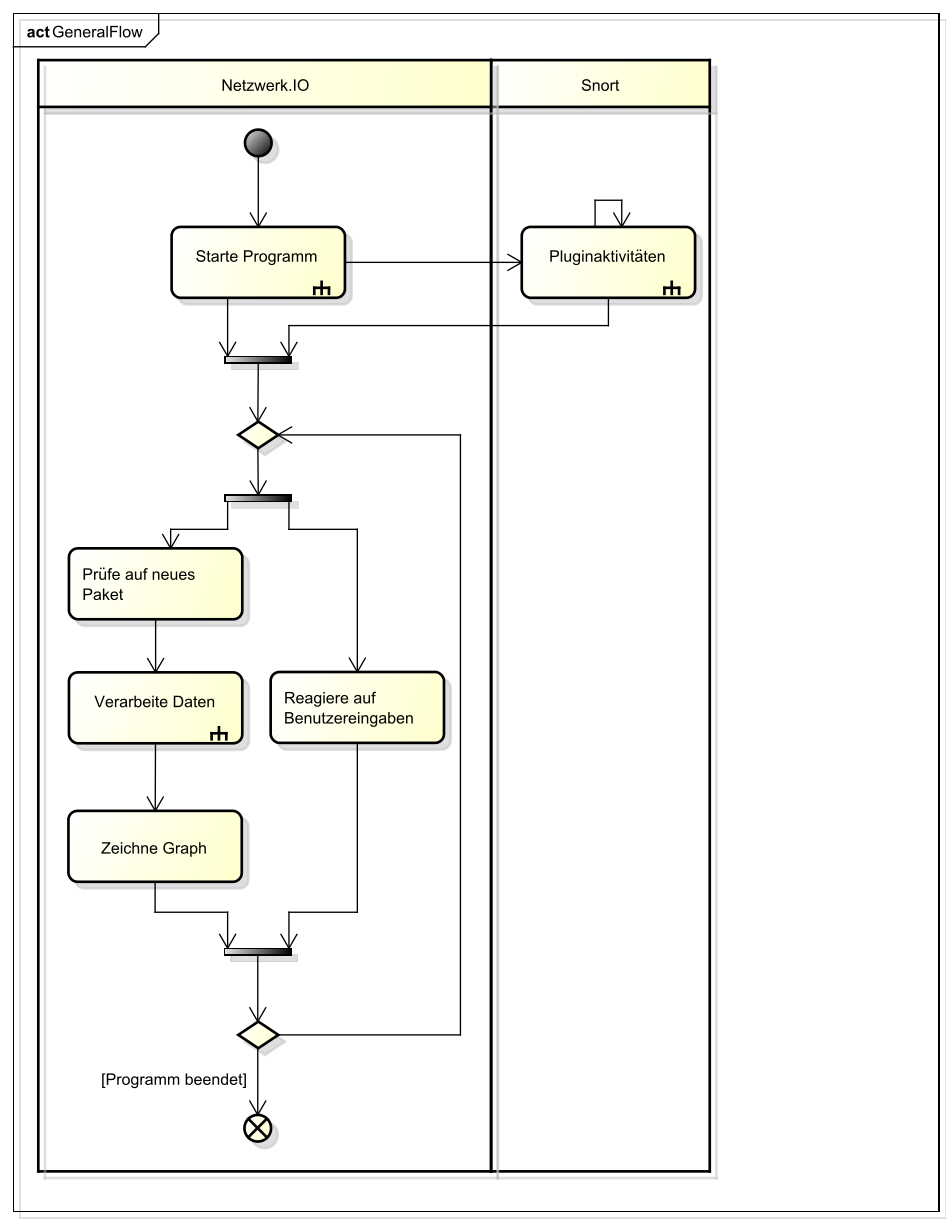
\includegraphics[width=\textwidth]{GeneralFlow}

\section{Anwendungsfälle} 

\chapter{GUI}

\section{Hauptfenster}
Die grafische Benutzeroberfläche ist vollbildoptimiert, lässt sich aber auch in
Fenstern skaliert anzeigen. Interaktion mit dem Benutzer findet über Hotkeys,
Mausposition und -klicks statt.
Die GUI ist standardmäßig auf Englisch.

  \begin{figure}[h!]
    \hspace*{0.15cm}\includegraphics[scale=0.07]{./img/GUI.png}
    \caption{Die grafische Benutzeroberfläche für \programname}
  \end{figure}

\noindent \textbf{Hintergrund:} Der Netzgraph wird im Hintergrund dauerhaft dargestellt und
aktualisiert. Standardmäßig wird nur dieser dargestellt und er ist für die
dauerhafte, interaktionslose Anzeige auf Status- oder Präsentationsdisplays
optimiert.
\\ \\
\textbf{Mittelgrund:} Einstellungsfenster, Filterfenster und optionales Statistikfenster
werden freischwebend über den Graph dargestellt und können verschoben und
geschlossen werden. Grundlegende Daten zum Graphen und Knoten werden an fester
Position als Overlay über dem Grahen angezeigt.
\\ \\
\textbf{Vordergrund:} Alarmfenster werden über allen anderen Fenstern angezeigt und
verschwinden nach Interaktion.

\section{Einstellungsfenster}
Das Einstellungsfenster dient zur Regelung der Einstellungen. Hier kann
beispielsweise die darstellung des Graphen angepasst werden, verschiedene
Graphalgorithmen ausgewählt werden etc.

  \begin{figure}[h!]
    \hspace*{0.3cm}\includegraphics[scale=0.07]{./img/Preferences.png}
    \caption{Das Einstellungsfenster von \programname}
  \end{figure}

\newpage
\section{Filterfenster}
Das Filtermenu erleichtert dem Benutzter die Beobachtung gewuenschter Knoten
durch die Hervorhebung dieser. Zum Beispiel können mit dem Namenfilter alle
Knoten die einen gemeinsamen Substring enthalten gefunden werden. In diesem
Bild werden alle Siemens Maschinen gefunden.

\begin{figure}[h!]
  \hspace*{0.2cm}\includegraphics[scale=0.06]{./img/Filters.png}
  \caption{Das Filterfenster von \programname}
\end{figure}


\appendix
\input{appendix}

\end{document}
